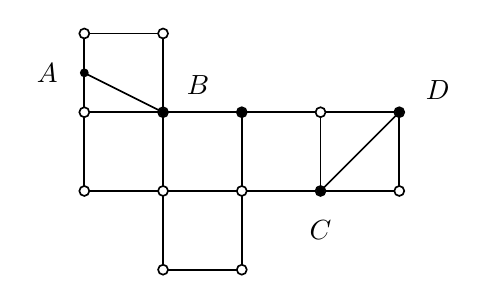
\begin{tikzpicture}[x=1cm,y=1cm,line width=.6pt,font=\normalsize]
% Cube net, unit squares; schematic projection of unfolding (schematic)
\coordinate (G00) at (0,0);
\coordinate (G10) at (1,0);
\coordinate (G20) at (2,0);
\coordinate (G30) at (3,0);
\coordinate (G40) at (4,0);
\coordinate (G01) at (0,1);
\coordinate (G11) at (1,1);
\coordinate (G21) at (2,1);
\coordinate (G31) at (3,1);
\coordinate (G41) at (4,1);
\coordinate (G02) at (0,2);
\coordinate (G12) at (1,2);
\coordinate (G0m1) at (1,-1);
\coordinate (G1m1) at (2,-1);
\coordinate (A) at (0,1.5);
\coordinate (B) at (1,1);
\coordinate (R) at (2,1);
\coordinate (C) at (3,0);
\coordinate (D) at (4,1);
% net squares
\draw (G00)--(G10)--(G11)--(G01)--cycle;
\draw (G10)--(G20)--(G21)--(G11)--cycle;
\draw (G20)--(G30)--(G31)--(G21)--cycle;
\draw (G30)--(G40)--(G41)--(G31)--cycle;
\draw (G01)--(G11)--(G12)--(G02)--cycle;
\draw (G10)--(G20)--(G1m1)--(G0m1)--cycle;
% segments AB and CD
\draw (A)--(B);
\draw (C)--(D);
% grid corner markers (open circles)
\foreach \p in {G00,G10,G20,G30,G40,G01,G11,G21,G31,G41,G02,G12,G0m1,G1m1} {\draw[fill=white] (\p) circle (1.8pt);}
% special points (filled)
\foreach \p in {A,B,R,C,D} {\fill (\p) circle (1.6pt);}
% labels with clearance
\node[anchor=east,xshift=-6pt] at (A) {$A$};
\node[anchor=west,xshift=5pt,yshift=10pt] at (B) {$B$};
\node[anchor=north,yshift=-7pt] at (C) {$C$};
\node[anchor=west,xshift=6pt,yshift=8pt] at (D) {$D$};
\end{tikzpicture}
